\documentclass[aspectratio=169,9pt,dvipsnames]{beamer}
\usetheme{Boadilla}

\usepackage[utf8]{inputenc}
\usepackage[english]{babel}
\usepackage[T1]{fontenc}

\usepackage{xcolor}
\usepackage{amsmath}
\usepackage{amsfonts}
\usepackage{amssymb}
\usepackage{graphicx}
\usepackage{changepage}
\usepackage{ragged2e}
\usepackage{amsmath,amssymb}
\usepackage{eurosym}
\usepackage{hyperref}
\usepackage{multicol}
\usepackage{caption}
\usepackage{subcaption}
\captionsetup{justification   = raggedright,
              singlelinecheck = false}
\usepackage[export]{adjustbox}

%\usepackage[toc,page]{appendix}
\usepackage{appendixnumberbeamer}
\usepackage{amssymb}% http://ctan.org/pkg/amssymb
\usepackage{pifont}% http://ctan.org/pkg/pifont
\newcommand{\cmark}{\ding{51}}%
\newcommand{\xmark}{\ding{55}}%

\usepackage{array,multirow,makecell}
\setcellgapes{1pt}
\makegapedcells
\newcolumntype{R}[1]{>{\raggedleft\arraybackslash }b{#1}}
\newcolumntype{L}[1]{>{\raggedright\arraybackslash }b{#1}}
\newcolumntype{C}[1]{>{\centering\arraybackslash }b{#1}}

\newcommand{\compresslist}{%
\setlength{\itemsep}{1pt}%
\setlength{\parskip}{0pt}%
\setlength{\parsep}{0pt}%
}

\beamertemplatenavigationsymbolsempty

\setbeamercolor{structure}{fg=teal}
\setbeamertemplate{itemize item}[circle]
\setbeamertemplate{section in toc}[square]
\setbeamertemplate{subsection in toc}[square]
\setbeamersize{text margin left=1cm, text margin right=1cm}
\setbeamertemplate{caption}[numbered]

\usepackage{lmodern}
\usefonttheme[onlymath]{serif}

\definecolor{teal_dark}{RGB}{26,140,140}



\justifying

\title[Climate survey - US]{\huge Climate survey - US}
\author[OECD]{OECD \\ \vspace{1cm}
     Results for the US: (partial) sample of 1,789 respondents (full will be 2,000).}% Representative along the \\gender, age, income, region and rural/urban dimensions but not representative along the education, ethnicity/race, vote and occupation dimensions. %\\Results are weighted along the gender, income, region, living in a metropolitan area, age, and race dimensions}
     % we don't use education, race nor vote as a quota, but it seems that highly educated and voters (and to a lesser extent, Biden voters) are over-represented, and Hispanic under-represented
%\author[Douenne \& \textbf{Fabre}]{\Large Thomas Douenne \& \textbf{Adrien Fabre} \large \\ $\quad$ \\ \textit{UvA (Amsterdam) \quad \textbf{ETH (Zurich)}}}
\date[\insertsection]{April 2021}





\begin{document}

	\begin{frame}

\titlepage
%\thispagestyle{empty}

	\end{frame}


\begin{frame}{Policy Effects}%
%\addtocounter{framenumber}{-1}
\vspace{-0.2cm}
\begin{figure}[h!]
\centering
\caption{Do you agree or disagree with the following statements? A carbon tax with cash transfers would…}
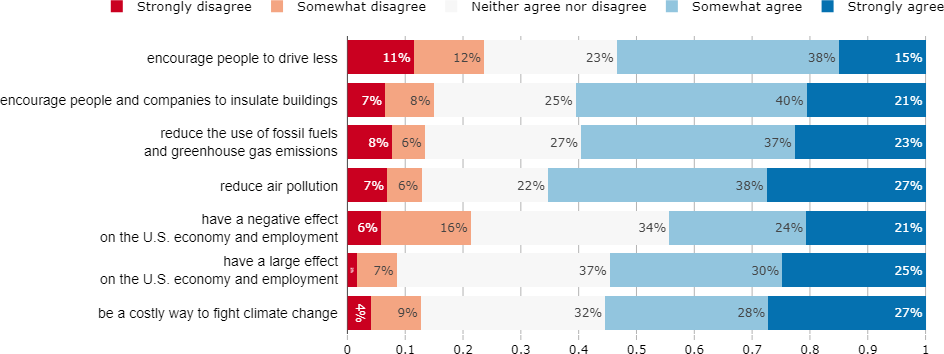
\includegraphics[width=.9\textwidth]{../figures/US/tax_transfers_effect_US.png}
%\caption{}
\end{figure}
\vspace{-0.2cm}
\begin{figure}[h!]


\centering
\caption{Do you support or oppose a carbon tax with cash transfers?}
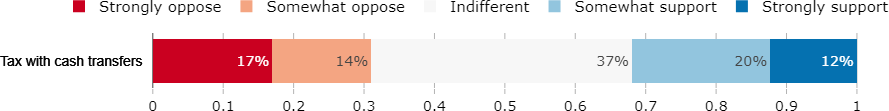
\includegraphics[width=.9\textwidth]{../figures/US/tax_transfers_support_US.png}
%\caption{}
\end{figure}
\end{frame}



\begin{frame}{Global climate politcs}%\addtocounter{framenumber}{-1}
\vspace{-0.2cm}
\begin{figure}
  \begin{minipage}[c]{0.3\textwidth}
		\caption{\small{At which level(s) do you think public policies to tackle climate change need to be put in place? (Multiple answers are possible)}}
  \end{minipage}\hfill
  \begin{minipage}[c]{0.67\textwidth}
    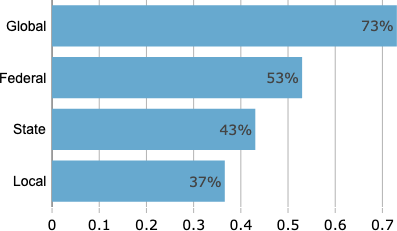
\includegraphics[width=.5\textwidth]{../figures/US/scale_US.png}
  \end{minipage}
\end{figure}


\begin{figure}[h!]
\centering
\caption{To achieve a given reduction of greenhouse gas emissions globally, costly investments are needed.
Ideally, how should countries bear the costs of fighting climate change?}
\vspace{2mm}
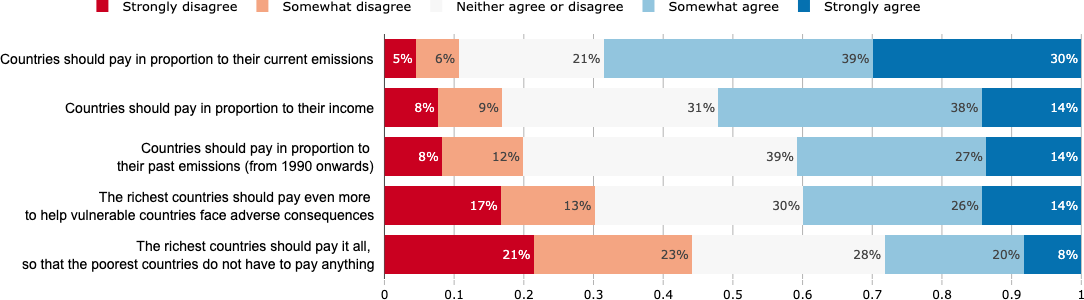
\includegraphics[width=.92\textwidth]{../figures/US/burden_sharing_US.png}
%\caption{}
\end{figure}
\end{frame}

\end{document}
